\section{Entire Polar Region}

In the following section, we apply the insights gained from local observations at \textit{AWIPEV} and \textit{Georg von Neumayer III} to the CRU data set.

The Diurnal Temperature Range (DTR) in the CRU dataset shows two regimes with differing trends. DTR values decline as monthly average temperatures increase in the regime below the freezing point, but increase again for average temperatures above \SI{0}{\celsius}. The slope of these declining and rising trends in the CRU data is smaller than the slopes for the local observations. Furthermore, the two regimes can be separated by a temperature barrier at \SI{0\pm0.5}{\celsius}, whereas for local observations at \textit{AWIPEV}, the data was separated at \SI{2\pm0.5}{\celsius}.

\begin{figure}[ht]
    \centering

    \begin{subfigure}[t]{0.45\textwidth}
        \centering
        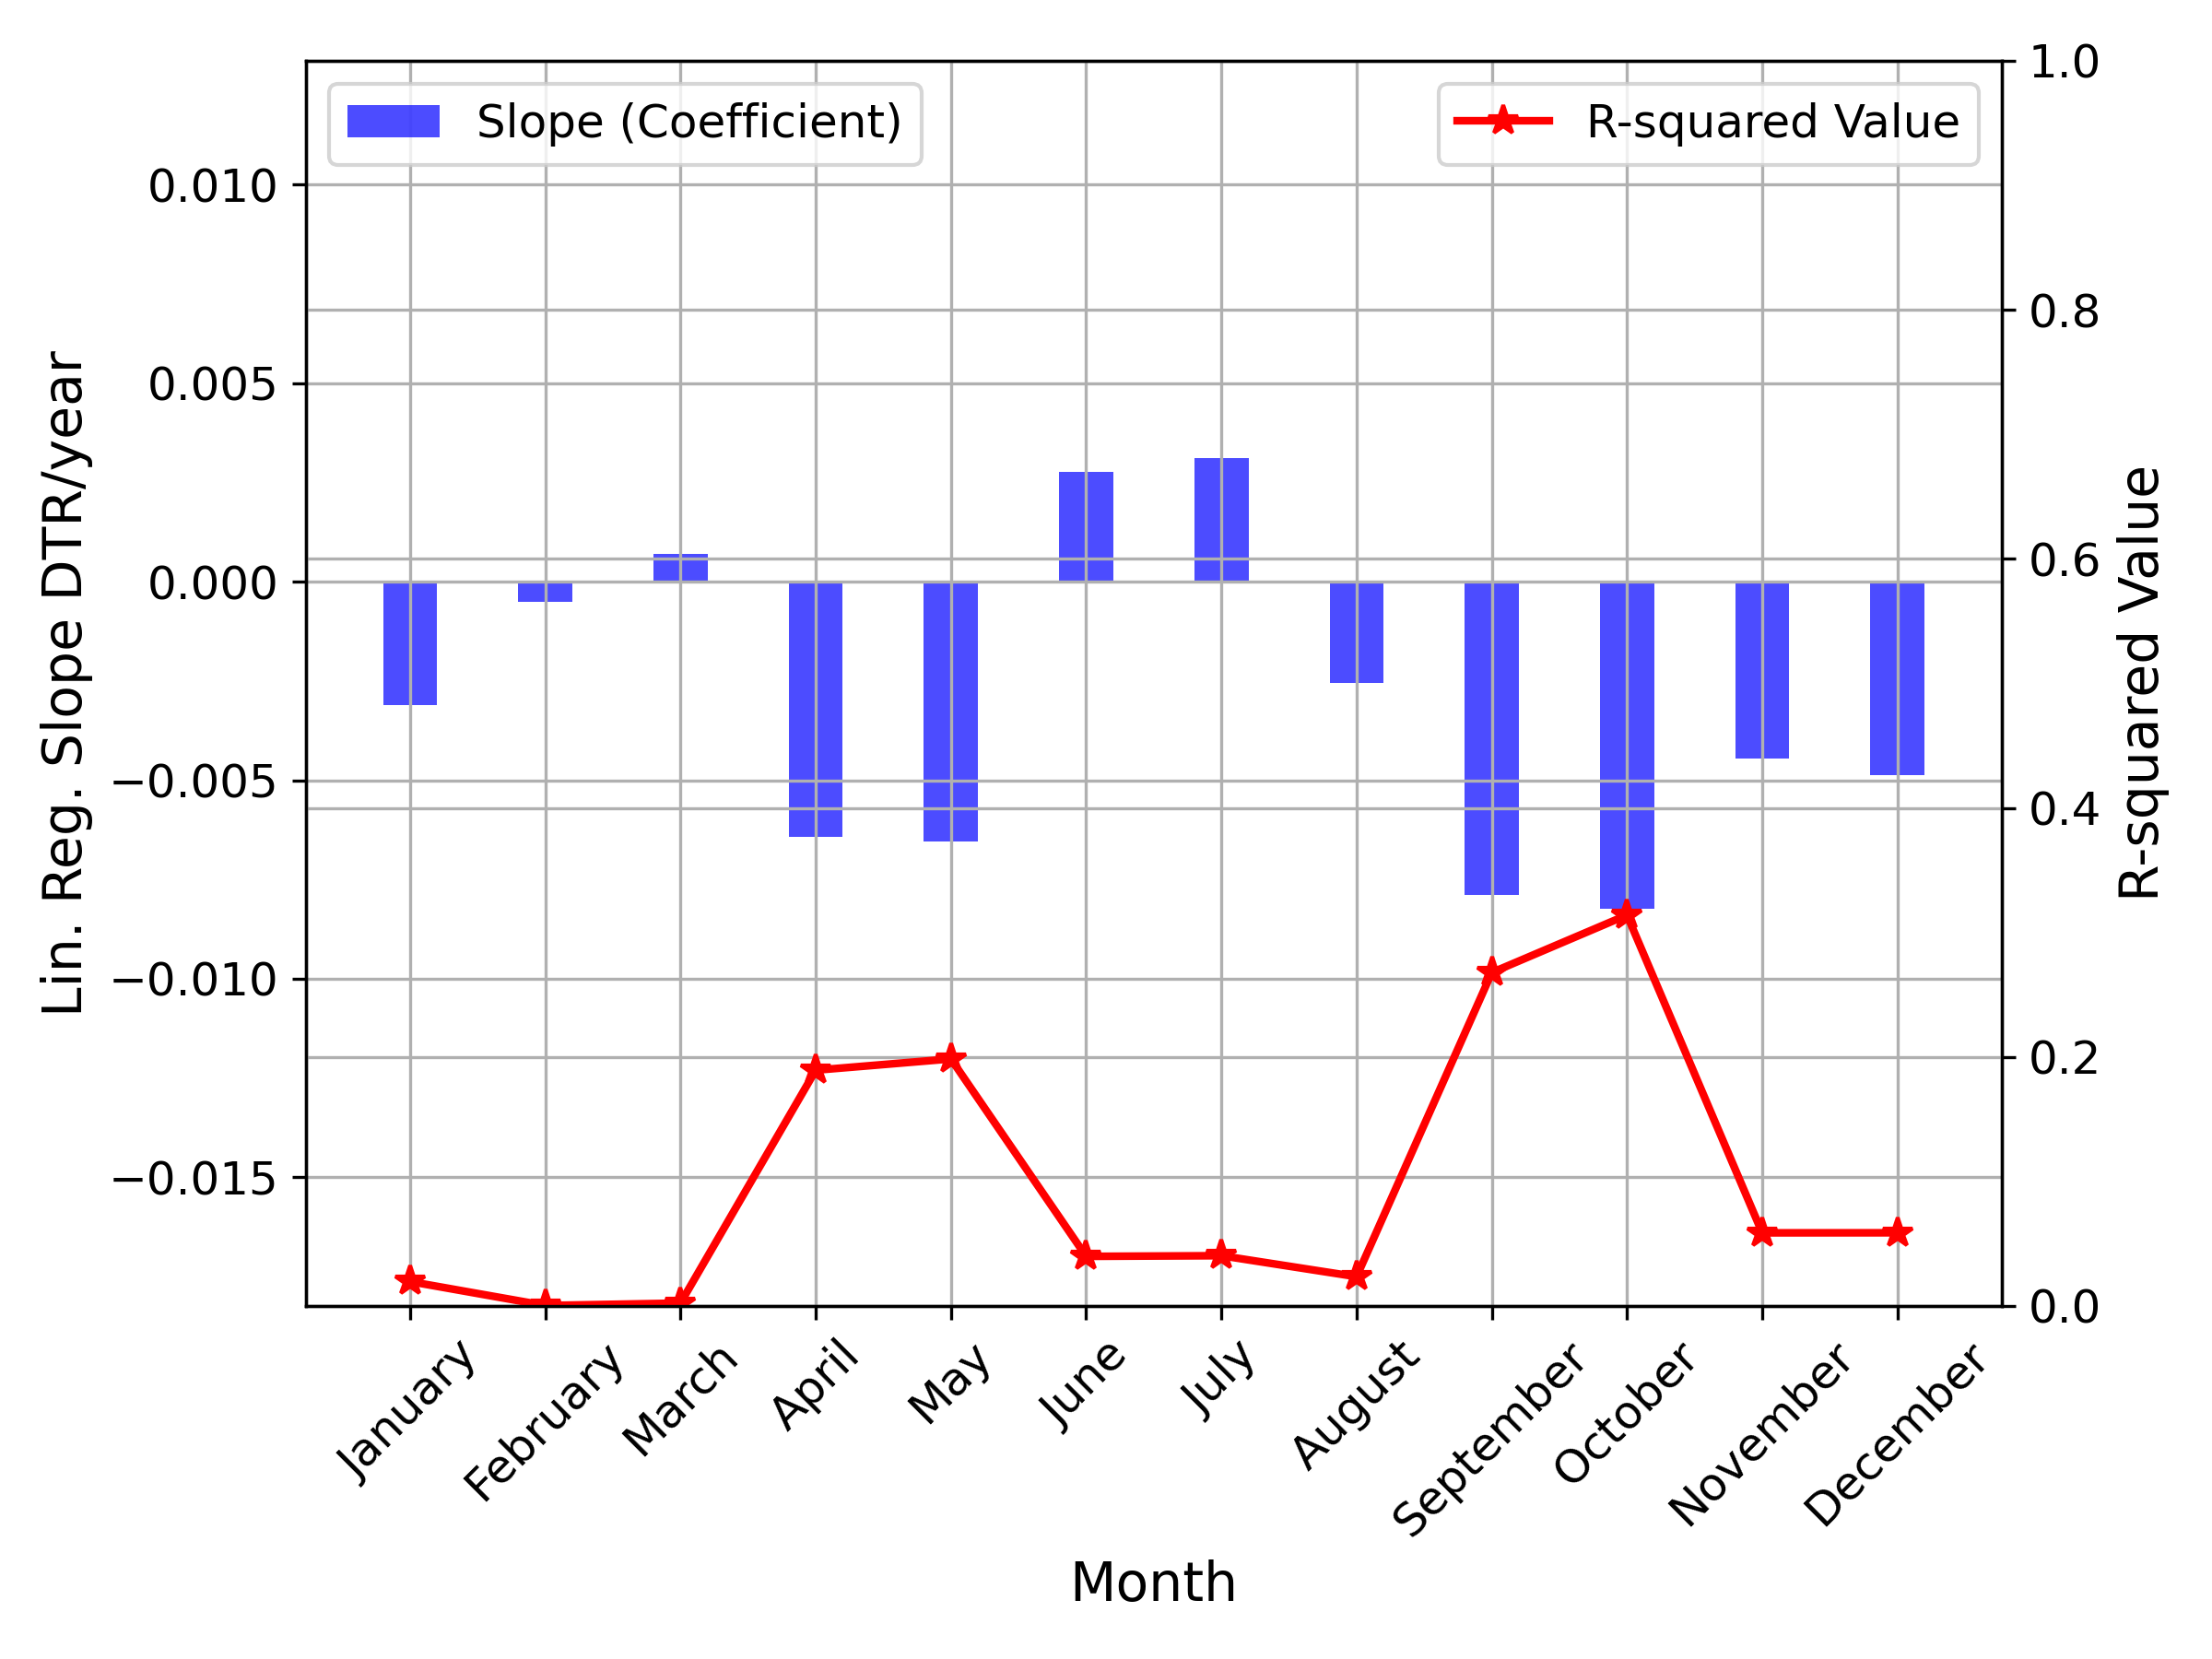
\includegraphics[width = \textwidth]{C:/Users/leonh/Desktop/Praktikum_AWI/DTR_R2_1973_2023.png}
        \caption{1973 - 2023}
    \end{subfigure}
    \hfil
    \begin{subfigure}[t]{0.45\textwidth}
        \centering
        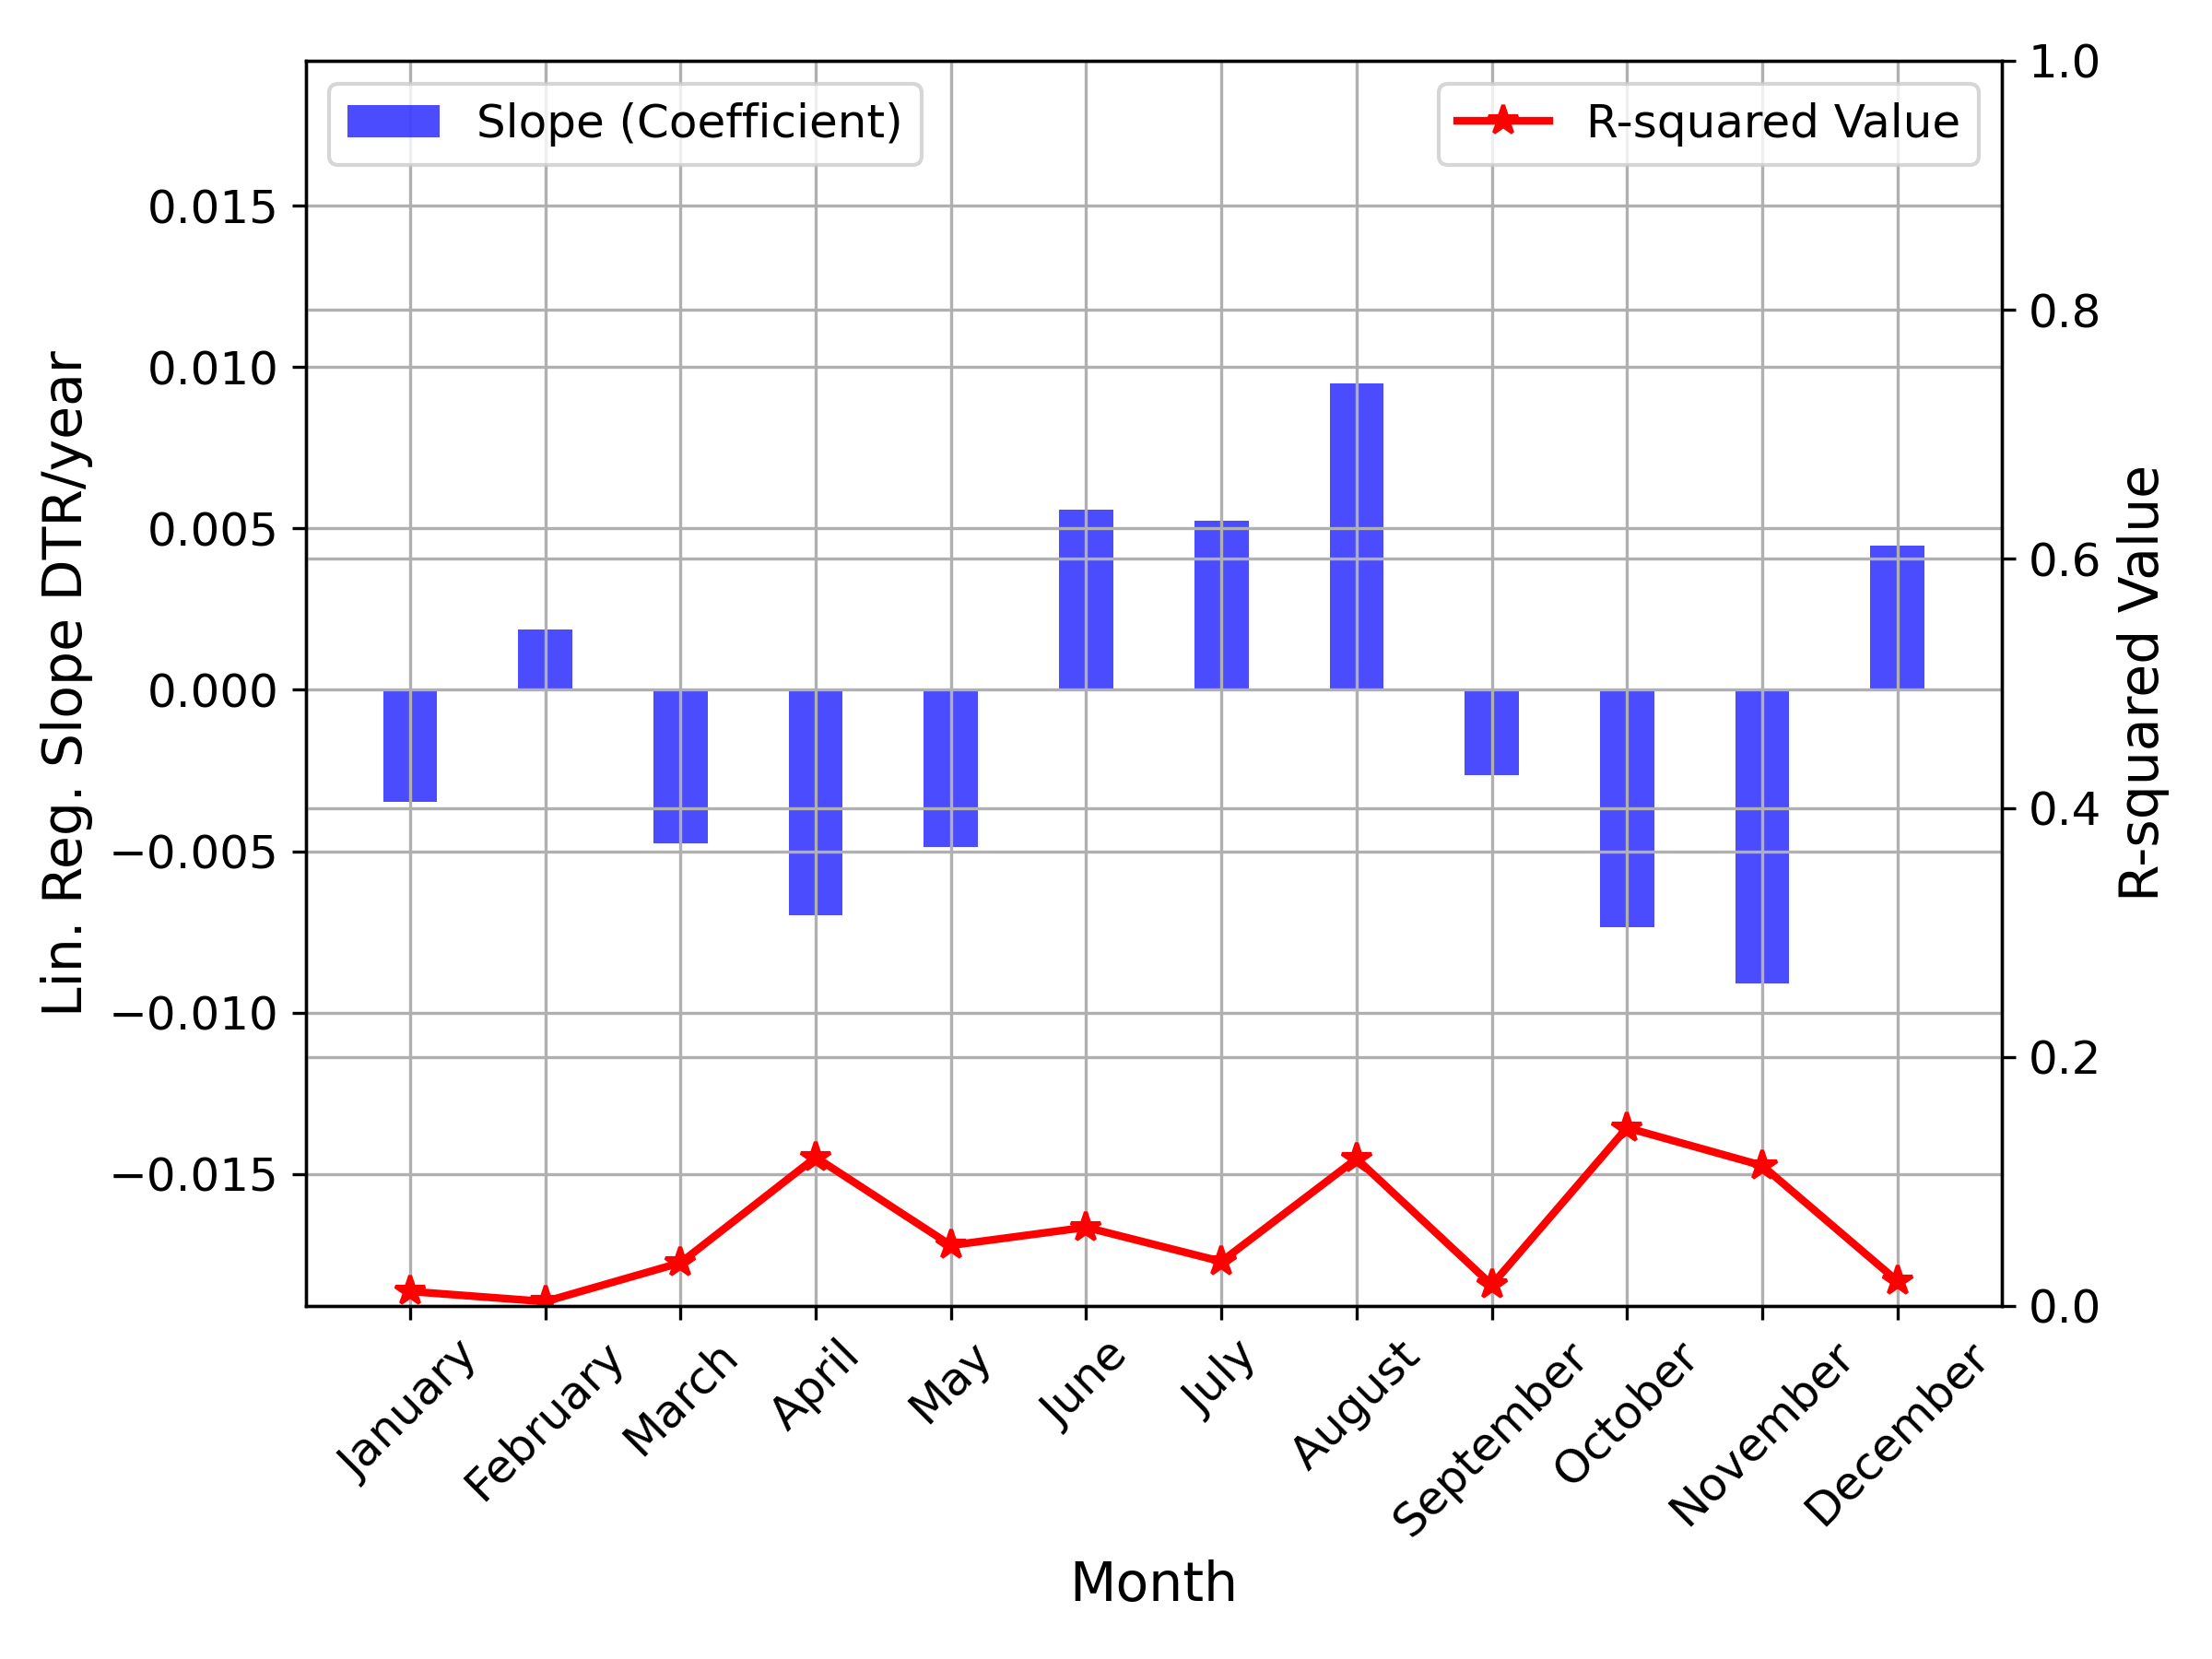
\includegraphics[width = \textwidth]{C:/Users/leonh/Desktop/Praktikum_AWI/DTR_R2_1993_2023.png}
        \caption{1993 - 2023}
    \end{subfigure}

    \caption{The DTR trend in the Arctic show rising trends in the summer.}
    \label{fig:2by2subfigures}
  \end{figure}

The smaller slopes are most likely an effect of averaging. In the following, we can make the smaller gradients plausible by introducing simplifying premises in a thought experiment: The spatially averaged temperature is generated by a normal distribution as the local influences are independent and random. Furthermore, the link between DTR and the average temperature at a local level is given by the relation examined in \cref{Sec:LocalDTRTrend}. It is assumed that the distributions do not change due to changes in the average temperature. In this case, the resulting DTR is a convolution of the average temperature distribution and the pattern connecting DTR and average temperature. As the convolution of two functions is always smoother than the initial function, the slope will be smaller than the initial slope.

The coefficient of determination, $R^2$, is smaller for the trends in DTR, with values at and below 0.2, than for the trends in average temperature.

As expected, we see an increase in DTR during June and August, contrary to the dominant trend. These two months fall into the second regime, characterized by temperatures above 0°C. As the Arctic continues to warm, the average temperature in more months is going to exceed 0°C. Therefore, the overall trend in DTR is likely to decelerate or even reverse.



